%!TEX root = ../../thesis.tex

In the short term future, CERN expects to operate Run II of the LHC in 2015 -- 2017, and 
Run III in 2019 -- 2021. Run II is designed to deliver \unit{\about100}{\invfb} at 
\unit{$\sqrt{s} = 13\text{ -- }14$}{\TeV}, whilst Run III is designed to deliver 
\unit{\about300}{\invfb} at \unit{$\sqrt{s} = 14$}{\TeV}. In the long term future, CERN 
plans to further upgrade the LHC instantaneous luminosity (HL-LHC), to start running in 
2023 and deliver \unit{\about3000}{\invfb} at \unit{$\sqrt{s} = 14$}{\TeV}.\footnote{
	Another post-LHC scenario is to upgrade the LHC energy to \unit{$\sqrt{s} = 33$}{\TeV} 
	(HE-LHC). Highly speculative longer term ideas include building a 
	\unit{100}{\kilo\metre} tunnel beneath Geneva to house a \unit{$\sqrt{s} = 1$}{\TeV} 
	\epluseminus collider (TLEP), and then later a \unit{$\sqrt{s} = 100$}{\TeV} \pp 
	collider. The international community is also considering proposals for \epluseminus 
	linear colliders, ILC and CLIC, which would have \unit{$\sqrt{s}~\about~1$}{\TeV}.
}

Compared to \unit{$\sqrt{s} = 8$}{\TeV}, the Higgs boson production cross sections at 
\unit{$\sqrt{s} = 14$}{\TeV} are \about2.5 times larger for ggF, VBF and \VH, and 
\about4.7 times larger for \ttH. Many of the background processes increase by a smaller 
factor, which should also aid the sensitivity of analyses. However, the harsher pile-up 
environment will degrade detector performance. These considerations, together with the 
large expected luminosities, yield more precise signal strength measurements and should 
enable rare decays (\eg \HepProcess{\PHiggs \HepTo \PZ\Pphoton} and \HepProcess{\PHiggs 
\HepTo \Pmu\Pmu}) and additional production channels (\eg \ttH) to be observed. Prospects 
for the \unit{300}{\invfb} and \unit{3000}{\invfb} datasets were investigated by ATLAS 
\cite{ATLAS:prospects}, and the expected precision of signal strengths and coupling scale 
factors are shown in \Figure~\ref{fig:concl:prospects}.

\begin{figure}[t]
	\begin{subfigure}[t]{0.495\textwidth}
		\centering
		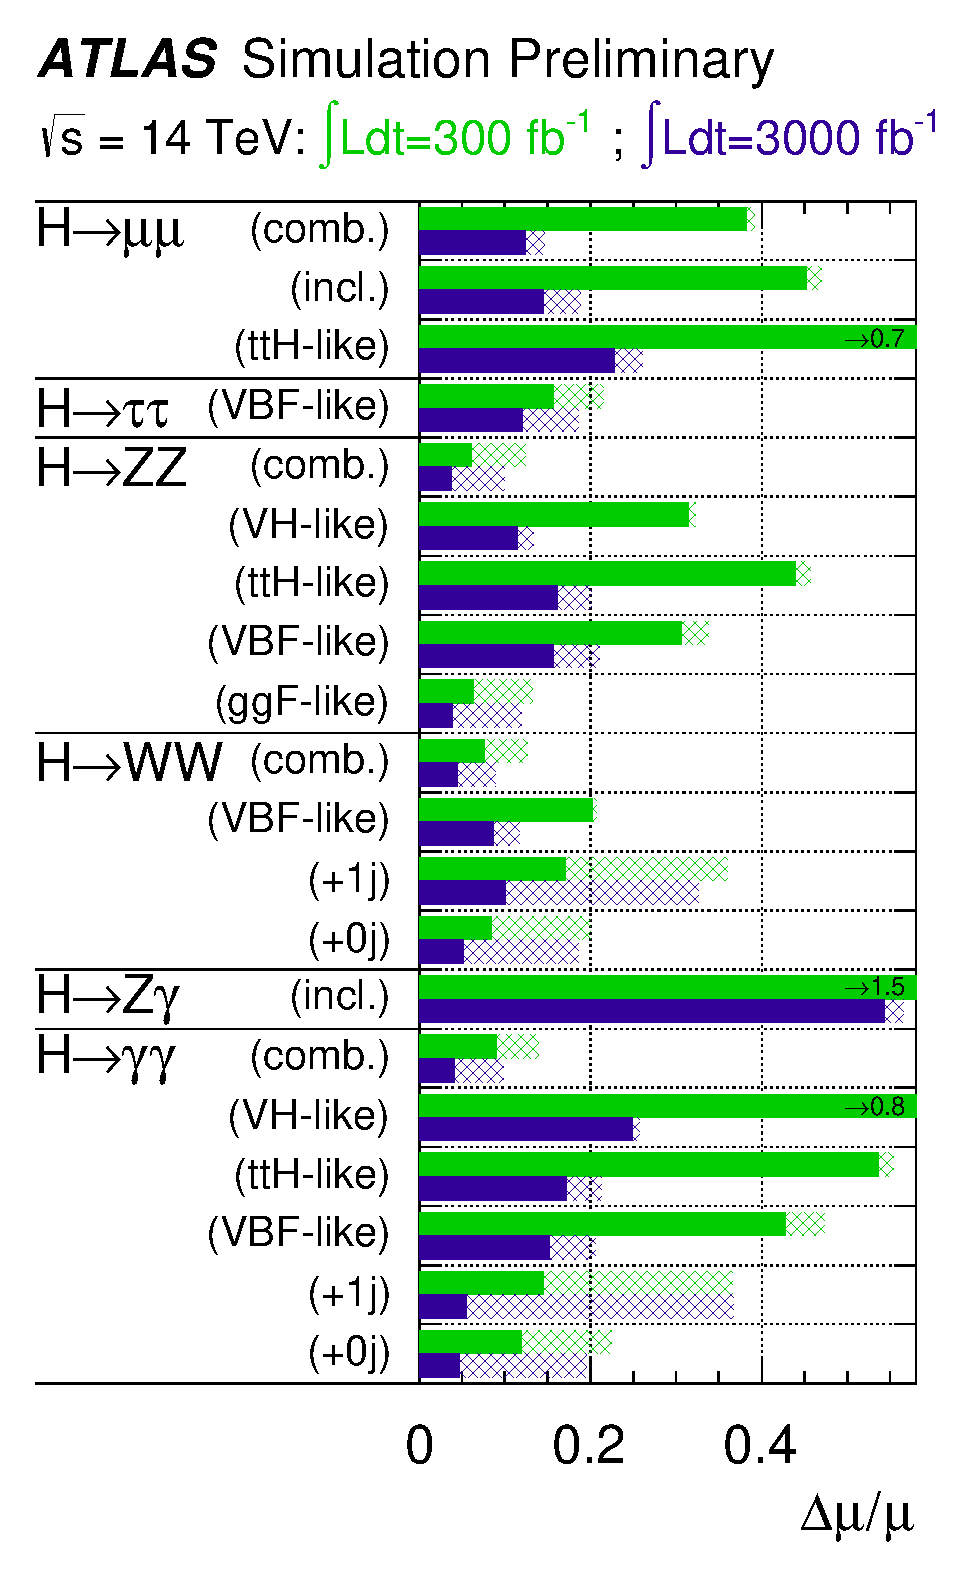
\includegraphics[width=\textwidth]{tex/conclusions/prospects_mu}
	\end{subfigure}
	\hfill
	\begin{subfigure}[t]{0.495\textwidth}
		\centering
		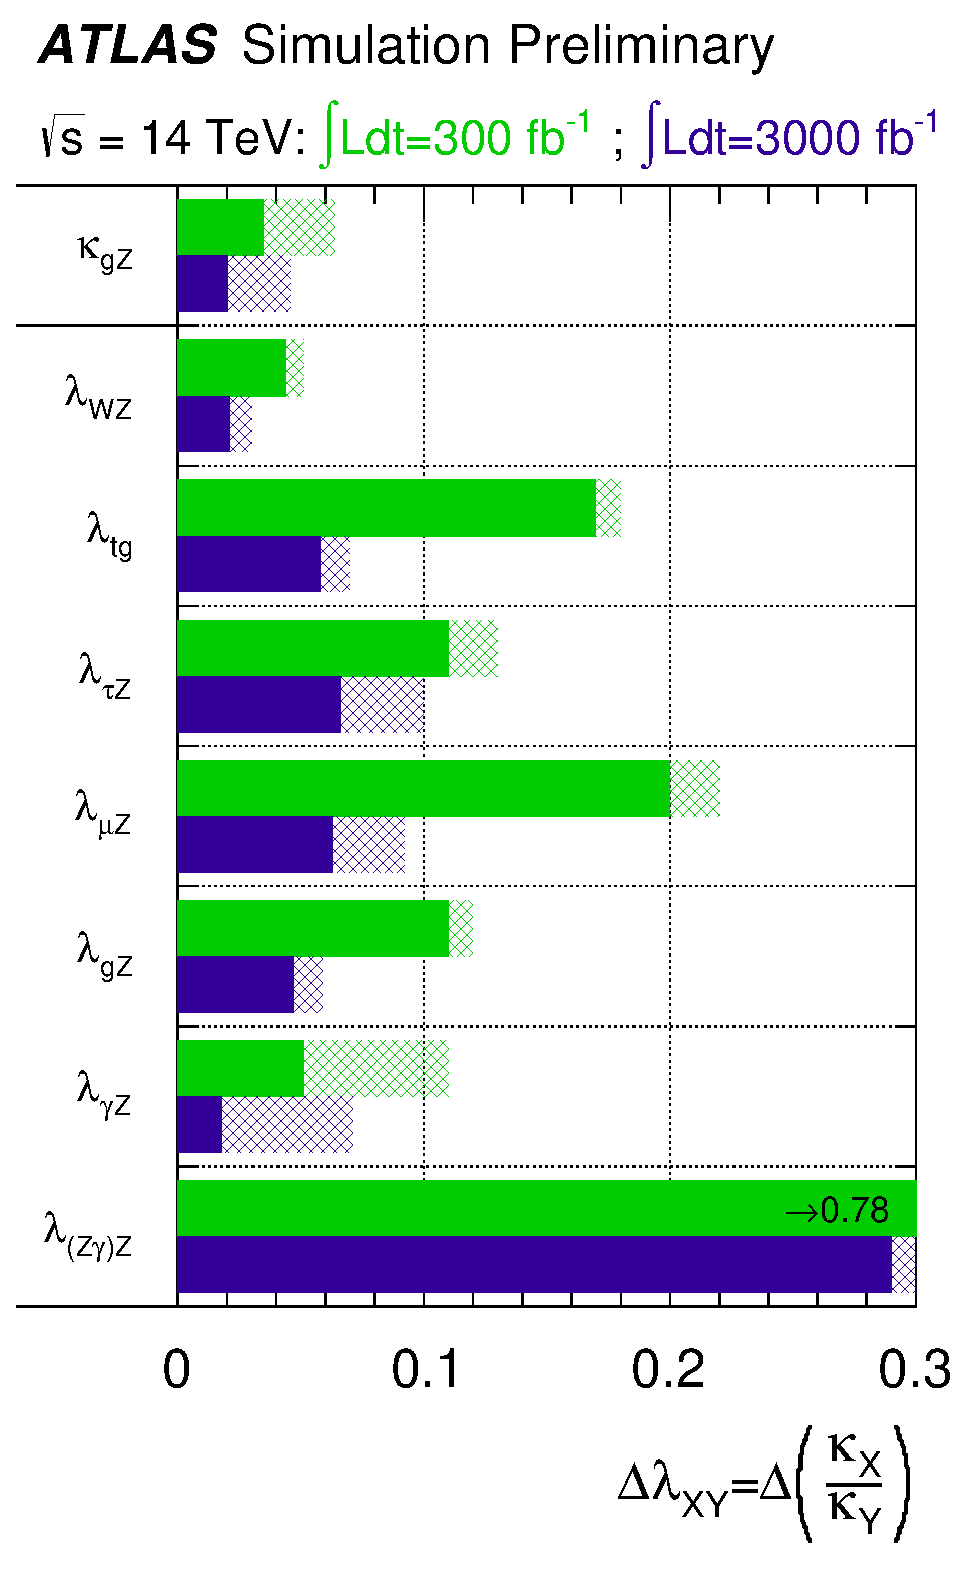
\includegraphics[width=\textwidth]{tex/conclusions/prospects_couplings}
	\end{subfigure}
	\caption{Expected precision of Higgs boson measurements at Run III of the LHC (green) 
	and the HL-LHC (blue), assuming \unit{$\mH = 125$}{\GeV} \cite{ATLAS:prospects}. The 
	left shows signal strength precision for a variety of experimental signatures. The 
	right shows the precision of coupling scale factor ratios, following the second 
	generic parametrisation described in \Section~\ref{sec:searches:couplings}. The hashed 
	areas indicate the decrease in precision due to theoretical uncertainties.}
	\label{fig:concl:prospects}
\end{figure}

The total width is predicted to be \unit{$\Gamma_{\PHiggs} = 4.07 \pm 0.16$}{\MeV} at 
\unit{$\mH = 125$}{\GeV} \cite{YR3}. Although this is not experimentally resolvable, it 
should be possible to indirectly constrain $\Gamma_{\PHiggs}$ at future LHC runs.
The Higgs boson propagator $1/((s^2 - m_{\PHiggs}^2)^2 + m_{\PHiggs}^2\Gamma_{\PHiggs}^2)$ 
indicates that the on-shell production cross section is sensitive to $\Gamma_{\PHiggs}$, 
though it is difficult to disentangle this information from coupling scale factors. 
However, by comparing the off-shell region to the on-shell region, it is possible to 
constrain $\Gamma_{\PHiggs}$ with \HepProcess{\PHiggs \HepTo \PZ\PZ} and \HWW events 
\cite{Caola:2013,Campbell:2013HZZ,Campbell:2013HWW}.
Also, interference between signal and continuum background can produce a 
$\Gamma_{\PHiggs}$-dependent shift in \mH, which could be measured at the HL-LHC with 
\HepProcess{\PHiggs \HepTo \Pphoton\Pphoton} events \cite{Dixon:2013,Martin:2013}.

At the HL-LHC it should be possible to measure diHiggs production, which would yield a 
first direct measurement of the Higgs self-coupling $\lambda$ \cite{DiHiggs}. This could 
prove important in understanding the metastability of the vacuum (see 
\Section~\ref{sec:implications:vacuum}). A measurement of triHiggs production would allow 
the final Higgs term in the Lagrangian to be measured, though is extremely experimentally 
challenging.

Finally, a solution to the hierarchy problem (see 
\Section~\ref{sec:implications:hierarchy}) shall be sought in future LHC runs. This is a 
very large topic in itself, though Higgs measurements will play their role in this. 
Additional (sometimes charged) Higgs bosons often feature in such models, and so searches 
for these shall continue. Also, it shall be important to further constrain the invisible 
Higgs width, which can act as a probe of dark matter candidates.

The discovery of the Higgs boson has initiated a new era in high energy physics. It 
confirms the Higgs mechanism of electroweak symmetry breaking, and appears to leave the 
Standard Model self-consistent and intact. However, it does present interesting 
opportunities to probe models of new physics.


